\chapter{Desarrollo del sistema}
\label{chap:desarrollo}

En este capítulo se describen cada uno de los objetivos definidos en el punto \ref{sec:objetivosEspecificos}, así como los retos y dificultades que han surgido y las diferentes decisiones de diseño que se han tomado.\\

El desarrollo del sistema, en cuanto al desarrollo del software, solo abarca desde el apartado \ref{obj3} hasta el final de este capítulo. El resto de apartados se refieren al estudio del problema.\\

El proceso de desarrollo del software objetivo de este \acs{TFG} ha sido mediante la definición de varios test que definieran la funcionalidad primero y después el desarrollo de las funciones que hicieran cumplir los test definidos. A lo largo de este capítulo se documentan los test definidos y las funciones que implementan las funcionalidades exigidas.\\


\section{Captura de requisitos}
\label{sec:requisitos}
En esta sección se explicarán los requisitos funcionales del proyecto y algunas consideraciones a tener en cuenta. \\

En la Tabla \ref{tab:reqFLASH} podemos ver un resumen de los requisitos pertenecientes a la gestión de la memoria.\\
 
\begin{table}[h!]
\centering
\begin{tabular}{p{.3\textwidth}p{.7\textwidth}}
\tabheadformat
  \tabhead{Atributo}   &
  \tabhead{Descripción}\\

Nombre:            & FLASH Driver                                                                                                                                                                                                                                                                                                                                           \\ \hline
Responsabilidades: & Abstraer del hardware del componente de almacenamiento en memoria FLASH, ofreciendo una interfaz de más alto nivel para operar con el mismo                                                                                                                                                                                                     \\ \hline
Colaboradores:     & FreeRTOS, FS Manager                                                                                                                                                                                                                                                                                                                            \\ \hline
Operaciones        & \begin{tabular}[c]{@{}l@{}}- Init --\textgreater Inicializar el hardware\\ - Reset --\textgreater Reinicia el hardware\\ - ReadFile --\textgreater Lee un archivos desde la memoria FLASH\\ - WriteFile --\textgreater Escribe un archivo en la memoria FLASH\\ - DeleteFile --\textgreater Elimina un archivo de la memoria FLASH\end{tabular} \\ \hline
\end{tabular}

\caption {Tabla resumen de requisitos de gestión de la memoria FLASH}
\label{tab:reqFLASH}
\end{table}

En la Tabla \ref{tab:reqGPS} podemos ver un resumen de los requisitos pertenecientes a la gestión del dispositivo GPS.\\

\begin{table}[h!]
\centering
\begin{tabular}{p{.3\textwidth}p{.7\textwidth}}
\tabheadformat
  \tabhead{Atributo}   &
  \tabhead{Descripción}\\
\hline
Nombre:            & GPS Driver                                                                                                                                      \\ \hline
Responsabilidades: & Abstraer del hardware del componente de geolocalización por GPS, ofreciendo una interfaz de más alto nivel para operar con el mismo      \\ \hline
Colaboradores:     & FreeRTOS, GPS Manager                                                                                                                    \\ \hline
Operaciones        & \begin{tabular}[c]{@{}l@{}}- Init --\textgreater Inicializar el hardware\\ - ReadGPS --\textgreater lee la posición del GPS\end{tabular} \\ \hline
\end{tabular}

\caption {Tabla resumen de requisitos de gestión del dispositivo GPS}
\label{tab:reqGPS}
\end{table}

En la Tabla \ref{tab:ReqFSManager} podemos ver un resumen de los requisitos pertenecientes al sistema de archivos.\\

\begin{table}[h!]
\centering
\begin{tabular}{p{.3\textwidth}p{.7\textwidth}}
\tabheadformat
  \tabhead{Atributo}   &
  \tabhead{Descripción}\\
  
\hline
Nombre:            & FS Manager                                                                                                                                                                                                                                                                                                                                                                                                                                                                                                                                         \\ \hline
Responsabilidades: & Gestionar las operaciones de persistencia con el sistema de archivos en memoria FLASH del sistema                                                                                                                                                                                                                                                                                                                                                                                                                                                  \\ \hline
Colaboradores:     & FreeRTOS, FLASH Driver, LOG module                                                                                                                                                                                                                                                                                                                                                                                                                                                                                                     \\ \hline
Operaciones        & \begin{tabular}[c]{@{}l@{}}- Init --\textgreater Inicializar el hardware\\ - Reset --\textgreater Reinicia el FS\\ - OpenFile --\textgreater Abre un archivo del FS\\ - CloseFile --\textgreater Cierra un archivo del FS\\ - ReadFile --\textgreater Lee N bytes de un archivo del FS\\ - WriteFile --\textgreater Escribe N bytes en un archivo del FS\\ - FeofFile --\textgreater Indica el final de un archivo del FS\\ - DeleteFile --\textgreater Elimina un archivo del FS\\ - NewFile --\textgreater Crea un archivo en el FS\end{tabular} \\ \hline
\end{tabular}

\caption {Tabla resumen de requisitos del manejador del sistema de archivos}
\label{tab:ReqFSManager}
\end{table}

En la Tabla \ref{tab:ReqGPSManager} podemos ver un resumen de los requisitos pertenecientes al manejador del dispositivo GPS.\\

\begin{table}[h!]
\centering
\begin{tabular}{p{.3\textwidth}p{.7\textwidth}}
\tabheadformat
  \tabhead{Atributo}   &
  \tabhead{Descripción}\\

\hline
Nombre:            & GPS Manager                                                                                                                                                                                       \\ \hline
Responsabilidades: & Gestionar las operaciones de geolocalización del sistema                                                                                                                                          \\ \hline
Colaboradores:     & FreeRTOS, GPS Driver, LOG module                                                                                                                                                      \\ \hline
Operaciones        & \begin{tabular}[c]{@{}l@{}}- Init --\textgreater Inicializar el hardware\\ - ReadGPS --\textgreater Lectura de las coordenadas GPS\\ - Send2Log --\textgreater Envío de datos al log\end{tabular} \\ \hline
\end{tabular}

\caption {Tabla resumen de requisitos del manejador del dispositivo GPS}
\label{tab:ReqGPSManager}
\end{table}

En la Tabla \ref{tab:reqLOG} podemos ver un resumen de los requisitos pertenecientes al módulo de gestión del LOG.\\

\begin{table}[h!]
\centering
\begin{tabular}{p{.3\textwidth}p{.7\textwidth}}
\tabheadformat
  \tabhead{Atributo}   &
  \tabhead{Descripción}\\

\hline
Nombre:            & LOG Module                                                                                                                                                                                                                                                                                                                            \\ \hline
Responsabilidades: & Realizar un log de las operaciones realizadas a través dela API del sistema                                                                                                                                                                                                                                                           \\ \hline
Colaboradores:     & FreeRTOS, FS Manager                                                                                                                                                                                                                                                                                                                  \\ \hline
Operaciones        & \begin{tabular}[c]{@{}l@{}}- Init --\textgreater Inicializar el módulo LOG\\ - Reset --\textgreater Reinicia el módulo LOG\\ - NewLog --\textgreater Crea un nuevo archivo de log\\ - DeleteLog --\textgreater Elimina un archivo de log\\ - WriteLog --\textgreater añade una entrada al archivo de log correspondiente\end{tabular} \\ \hline
\end{tabular}

\caption {Tabla resumen de requisitos del módulo de LOG}
\label{tab:reqLOG}
\end{table}

Además de los requisitos anteriormente citados, se deben aplicar los siguientes principios de diseño:
\begin{itemize}
\item Estructura del sistema basada en un modelo de capas. Muy común en el desarrollo de sistemas empotrados, ya que con una capa de abstracción del hardware se permite la adaptabilidad del sistema a otras plataformas con poco esfuerzo.
\item Uso de un sistema operativo robusto y confiable para sistemas empotrados. Debido a la complejidad del sistema y las capacidades de comunicación que debe ofrecer, se ha optado por el uso de un sistema operativo en lugar de una aplicación standalone, lo que mejora la robustez, flexibilidad, seguridad y capacidad de recuperación.\\
\end{itemize}

Se deben incluir también los requisitos no funcionales especificados en el capítulo \ref{chap:objetivos}: que el software sea extensible, robusto, flexible, con capacidad de recuperación ante errores y adaptable.\\

\section{Comprensión de la plataforma hardware}
\label{obj1}
El conocimiento de la plataforma hardware se centra especialmente es tres componentes: el dispositivo GPS, la memoria FLASH que tiene la placa y la placa en su conjunto para conocer cómo funciona la programación del dispositivo y la interacción con los otros dos componentes.\\

En la Figura \ref{fig:BlocksSTM32} podemos ver el diagrama de bloques de la placa utilizada.\\

\begin{figure}[!h]
\begin{center}
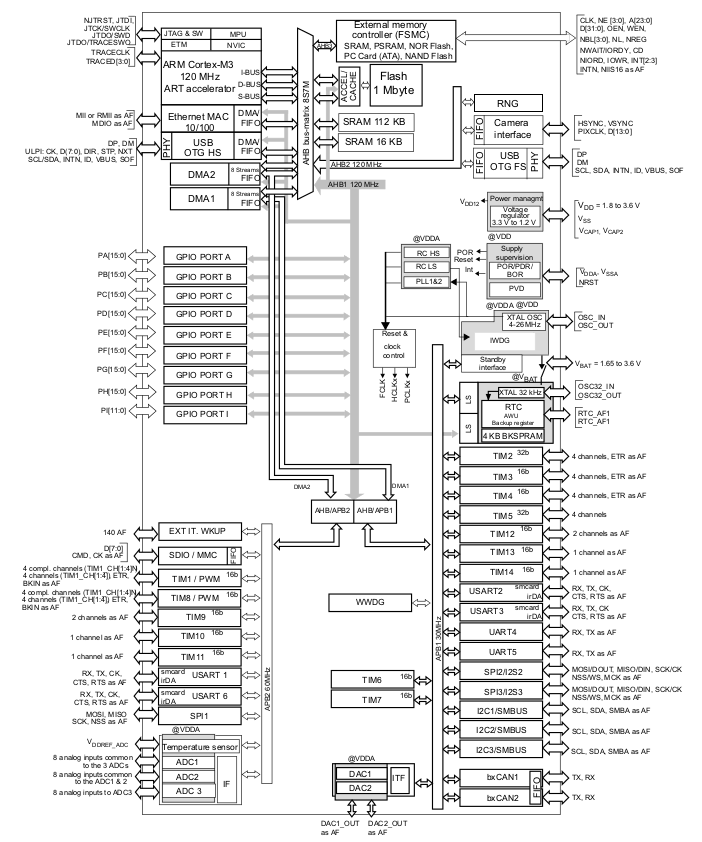
\includegraphics[width=0.5\textwidth]{figs/BlocksSTM32.png}
\caption{Diagrama de bloques de la placa STMF205VGT6}
\label{fig:BlocksSTM32}
\end{center}
\end{figure}

\subsection{Memoria FLASH}

En la Tabla \ref{tab:FLASHTable} podemos ver las características principales de la memoria FLASH \cite{bib:flash}.\\

\begin{table}[h!]
\centering
\begin{tabular}{p{.3\textwidth}p{.7\textwidth}}
\tabheadformat
  \tabhead{Atributo}   &
  \tabhead{Descripción}\\
\hline
Nombre:          & Memoria FLASH integrada                                                                                                                                                                                                                                                                                                                                                                                                                                                                                                                                                                                                                                                                                                                                                                                                                                                                                                                                        \\ \hline
Definido por:    & ST Microelectronics                                                                                                                                                                                                                                                                                                                                                                                                                                                                                                                                                                                                                                                                                                                                                                                                                                                                                                                                            \\ \hline
Documentación:   & \url{http://www.st.com/web/en/catalog/mmc/FM141/SC1169/SS1575/LN1433/PF245091}
\\ \hline
Características: & \begin{tabular}[c]{@{}l@{}}- Capacidad de 1 MByte.\\ - Soporta lecturas de hasta 128 bits en una única operación.\\ - Soporta escrituras de media, una o dos palabras. \\ - El tamaño de palabra es de 32 bits.\\ - Las operaciones de borrado o erase se pueden realizar a nivel\\   de sector físico o de toda la memoria al completo.\\ - Por defecto la escritura en memoria está deshabilitada.\\ - El estado de la FLASH se especifica en tiempo real \\   en el registro FLASH\_SR.\\ - La organización de los módulos de la memoria FLASH \\   se puede ver en la Tabla \ref{tab:org_FLASH}.\\ - La memoria de sistema es la que contiene el boot-loader.\\ - La memoria FLASH puede funcionar con voltaje entre 1.8V\\   y 3.6V, dividido en varios rangos y configurable.\\ - El voltaje de la FLASH puede afectar a la velocidad de la misma.\\ - Se puede configurar la latencia de la memoria FLASH y si queremos\\   o no prefetch de instrucciones.\end{tabular} \\ \hline
\end{tabular}

\caption {Tabla descripción de las características de la memoria FLASH}
\label{tab:FLASHTable}
\end{table}


El funcionamiento de una memoria FLASH tiene sustanciales diferencias con respecto a otro tipo de tecnologías de almacenamiento. Una memoria FLASH después de realizar una operación de \textit{Erase}, \textit{reset} o borrado tiene todos sus bits a 1 y a partir de ahí podemos escribir cualquier dato. Una vez escrito no podemos sobreescribirlo directamente, ya que esta tecnología no es capaz de cambiar un bit de un 0 a un 1 (sí de un 1 a un 0) mediante una operación de escritura. El cambio de cualquier bit de 0 a 1 se produce con la función Erase, cuya granularidad mínima es un sector físico completo y borra toda la información del mismo.\\

En la Tabla \ref{tab:org_FLASH} se puede ver la estructura interna de la memoria FLASH.\\

\begin{table}[h!]
\centering
%\begin{tabular}{llll}
\begin{tabular}{p{.2\textwidth}p{.2\textwidth}p{.2\textwidth}p{.2\textwidth}}
\tabheadformat
  \tabhead{Bloque}   &
  \tabhead{Nombre}      &
  \tabhead{Dirección del bloque} &
  \tabhead{Tamaño}  \\
\hline
%\textbf{Bloque}                        &\textbf{Nombre}& \textbf{Dirección del bloque}& \textbf{Tamaño}    \\ \hline
\multirow{9}{*}{Memoria principal}     & Sector 0      & 0x0800 0000\newline 0x0800 3FFF & 16 KByte  \\ \cline{2-4} 
                                       & Sector 1      & 0x0800 4000\newline 0x0800 7FFF & 16 KByte  \\ \cline{2-4} 
                                       & Sector 2      & 0x0800 8000\newline 0x0800 BFFF & 16 KByte  \\ \cline{2-4} 
                                       & Sector 3      & 0x0800 C000\newline 0x0800 FFFF & 16 KByte  \\ \cline{2-4} 
                                       & Sector 4      & 0x0801 0000\newline 0x0801 FFFF & 64 KByte  \\ \cline{2-4} 
                                       & Sector 5      & 0x0802 0000\newline 0x0803 FFFF & 128 KByte \\ \cline{2-4} 
                                       & Sector 6      & 0x0804 0000\newline 0x0805 FFFF & 128KByte  \\ \cline{2-4} 
                                       & ...           & ...                       & ...       \\ \cline{2-4} 
                                       & Sector 11     & 0x080E 0000\newline 0x080F FFFF & 128 KByte \\ \hline
\multicolumn{2}{l}{Memoria de sistema}               & 0x1FFF 0000\newline 0x1FFF 77FF & 30 KByte  \\ \hline
\multicolumn{2}{l}{Area OTP (one-time programmable)} & 0x1FFF 7800\newline 0x1FFF 7A0F & 528 Bytes \\ \hline
\multicolumn{2}{l}{Bytes de opciones}                & 0x1FFF C000\newline 0x1FFF C00F & 16 Bytes  \\ \hline
\end{tabular}

\caption {Organización de los módulos de la memoria FLASH}
\label{tab:org_FLASH}
\end{table}

Para hacernos una idea de la restricción que supone tener sectores de hasta 128 KBytes, que funcionan como un ente indivisible para la función de borrado/erase, el disco duro de estado sólido SSDSA1MH080G1 de Intel, que funciona con la misma tecnología, tiene un tamaño de sector de 512 Bytes \cite{bib:intelssd}.\\

Además una memoria FLASH especifica su ciclo de vida en el número de operaciones de borrado que se pueden realizar, típicamente entre 100.000 y 1.000.000.\\


\subsection{Dispositivo GPS}
\label{sec:dispGPS}
En la Tabla \ref{tab:GPSTable} podemos ver las características principales del dispositivo GPS \cite{bib:gps}.\\

\begin{table}[h!]
\centering
\begin{tabular}{p{.3\textwidth}p{.7\textwidth}}
\tabheadformat
  \tabhead{Atributo}   &
  \tabhead{Descripción}\\

\hline
Nombre:          & PA6H GPS Module                                                                                                                                                                                                                                                                                                                                                                                                                                                                                                                                                                                                                                                                                                                                                                                                                                             \\ \hline
Definido por:    & GlobalTop Technology                                                                                                                                                                                                                                                                                                                                                                                                                                                                                                                                                                                                                                                                                                                                                                                                                                        \\ \hline
Documentación:   & \url{http://www.gtop-tech.com/en/product/PA6H-GPS-Module/MT3339\_GPS\_Module\_04.html}
\\ \hline
Características: & \begin{tabular}[c]{@{}l@{}}- Chipset Mediatek MT3339.\\ - Antena GPS integrada con soporte para antena externa.\\ - Alta sensibillidad -165dBm, diseño TCXO.\\ - Soporte DPGS (WAAS/EGNOS/MASA/GAGAN).\\ - Precisión de 3 metros.\\ - Soporte protocolos NMEA 0183 y PMTK.\\ - Conectado a la placa a través de la USART 3.\end{tabular} \\ \hline

\end{tabular}

\caption {Tabla descripción de las características del dispositivo GPS}
\label{tab:GPSTable}
\end{table}

Fundamentalmente el factor de mayor importancia del dispositivo GPS es cómo realiza la comunicación con el resto del sistema y cómo podemos comunicarnos con él y cómo configurarlo.\\

No es necesario centrarse en la configuración de los pines de entrada/salida del dispositivo GPS ya que está integrado en la misma placa donde están integrados el resto de dispositivos.\\

Sobre la codificación de los datos que nos proporciona el GPS se ha decido utilizar el estándar de la \acf{NMEA} \cite{bib:commandGPS}.\\

\acs{NMEA} es un estándar de codificación de datos que proporciona una especificación de cómo deben codificarse los datos de diversos dispositivos electrónicos como pueden ser el GPS, sónar, radar, giroscopio, anemómetro, etc. Este estándar documenta multitud de diferentes tipos de mensajes para muy diferentes componentes. La forma de normalizar todos estos mensajes es mediante una cadena de control que comienza con el símbolo del dólar (\$), seguido de un identificador del dispositivo de dos caracteres(GP en el caso del GPS) al que acompaña un identificador de tres caracteres del dato al que se refiere el mensaje. A partir de ahí, y separados por comas, se suceden todos los datos que correspondan a un paquete de datos. El final del mensaje de este protocolo es un símbolo de asterisco (*) seguido de una suma de control de los datos y los caracteres <CR><LF> de fin de mensaje \cite{bib:nmea}.\\

Con respecto al dispositivo GPS solo se tendrán en cuenta los datos que ofrece, ya que la configuración por defecto sirve para el propósito planteado. De los datos que ofrece solo interesarían los identificados por los caracteres GGA, que hacen referencia a los <<Datos Corregidos del Sistema de Posicionamiento GLobal>>. Este mensaje proporciona la posición, separada en longitud, latitud y altura sobre el nivel del mar; el tiempo UCT en el que se generó el mensaje; y si se ha aplicado algún factor de corrección. Se puede ver un ejemplo de mensaje y el significado de los diversos campos en la Tabla \ref{tab:GPS_Data}.\\

\begin{table}[h!]
\centering

\begin{tabular}{p{.3\textwidth}p{.2\textwidth}p{.4\textwidth}}
\tabheadformat
  \tabhead{Nombre}   &
  \tabhead{Ejemplo}      &
  \tabhead{Descripción}  \\
\hline
%\textbf{Nombre}          & \textbf{Ejemplo} & \textbf{Descripción}                                                                               \\ \hline
Identificador de mensaje & \$GPGGA          & Cabecera del protocolo GGA                                                                         \\ \hline
Tiempo UTC               & 064951.000       & hhmmss.sss                                                                                         \\ \hline
Latitud                  & 2307.1256        & ddmm.mmmm                                                                                          \\ \hline
Indicador N/S            & N                & N=norte, S=sur                                                                                     \\ \hline
Longitud                 & 12016.4438       & dddmm.mmmm                                                                                         \\ \hline
Indicador E/O            & E                & E=este, W=oeste                                                                                    \\ \hline
Indicador de posición    & 1                & \begin{tabular}[c]{@{}l@{}}0=no disponible, 1=ajustado,\\  2=diferente ajuste del GPS\end{tabular} \\ \hline
Nº de satélites usados   & 8                & Entre 0 y 14                                                                                       \\ \hline
HDOP                     & 0.95             & Dilución de la precisión horizontal                                                                \\ \hline
Altitud sobre el mar     & 39.9             & \begin{tabular}[c]{@{}l@{}}Altitud, en metros, de la antena \\ sobre el nivel del mar\end{tabular} \\ \hline
Unidades                 & M                & Metros de altitud de la antena                                                                     \\ \hline
Separación geoidal       & 17.8             &                                                                                                    \\ \hline
Unidades                 & M                & Metros de la separación geoidal                                                                    \\ \hline
Age of Diff. Corr.       &                  & \begin{tabular}[c]{@{}l@{}}Nulo cuando no se utiliza DGPS\\  en segundos\end{tabular}              \\ \hline
Checksum                 & *65              &                                                                                                    \\ \hline
CR LF                    &                  & Fin de mensaje                                                                                     \\ \hline
\end{tabular}


\caption {Estructura de los datos porporcionados por el GPS}
\label{tab:GPS_Data}
\end{table}


\subsection{Placa STMF205VGT6}
Sobre la placa objetivo, al igual que se ha hecho con el GPS, solo se describirán aquellos aspectos que son relevantes para la realización de este TFG, se puede ver en la Tabla \ref{tab:BoardTable} \cite{bib:datasheet}.\\


\begin{table}[h!]
\centering
\begin{tabular}{p{.3\textwidth}p{.7\textwidth}}
\tabheadformat
  \tabhead{Atributo}   &
  \tabhead{Descripción}\\

\hline
Nombre:          & STMF205VGT6                                                                                                                                                                                                                                                                                                                                                                                                                                                                                                                                                                                                                                                                                                                                                                                                                                                 \\ \hline
Definido por:    & ST Microelectronics                                                                                                                                                                                                                                                                                                                                                                                                                                                                                                                                                                                                                                                                                                                                                                                                                                         \\ \hline
Documentación:   & \url{http://www.st.com/web/en/catalog/mmc/FM141/SC1169/SS1575/LN1433/PF245091} \\ \hline
Características: & \begin{tabular}[c]{@{}l@{}}- Core ARM 32-bit Cortex-M3 CPU.\\ - 1024 KB FLASH Memory.\\ - 128 KB SRAM.\\ - Comunicaciones UART, USART, SPI, I2C, CAN, USB 2.0.\\ - DMAC.\\ - Tanto la memoria FLASH, como el procesador y las UART\\   y USART están conectadas entre sí gracias a una matriz de \\   buses AHB.\\ - Acelerómetro.\\ - 16 canales conversor analógico-digital.\\ - 2 canales conversor digital-analógico.\\ - Timers de 16 y 32 bits.\\ - Oscilador interno de 32 KHz, uno de cristal de 4 a 20 MHz.\\ - Debug serie (SWD), JTAG y Cortex-M3 Trace.\\ - Generador de números aleatorios.\\ - 3 modos de arranque: desde FLASH, desde memoria de \\   sistema o desde SRAM.\\ - El boot-loader está en la memoria de sistema y sirve para\\   reprogramar la FLASH.\\ - Tiene un Controlador de interrupciones apiladas (NVIC).\end{tabular} \\ \hline
\end{tabular}
\caption {Cuadro descripción de las características de la placa STMF205VGT6}
\label{tab:BoardTable}
\end{table}


\section{Conocimiento software de acceso al hardware}
\label{obj2}
Una vez conocidos los componentes hardware  a utilizar y sus principales características, a continuación se describirán las bibliotecas de funciones proporcionadas por el fabricante de los mismos.\\

En la Figura \ref{fig:LibraryArch} se puede ver el diagrama estructural de la biblioteca del fabricante dividida en las diferentes capas que la componen.\\

\begin{figure}[!h]
\begin{center}
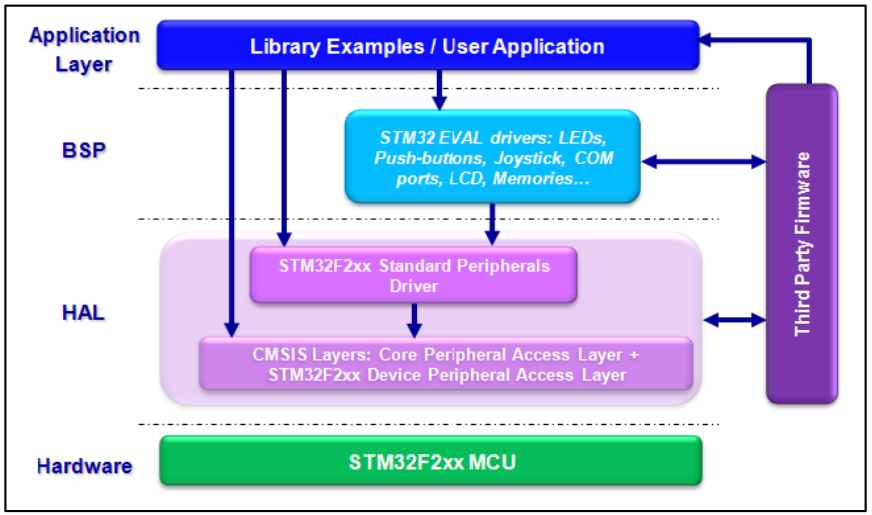
\includegraphics[width=1\textwidth]{figs/LibraryArch.png}
\caption{Diagrama en capas de la organización de la biblioteca de funciones de la placa}
\label{fig:LibraryArch}
\end{center}
\end{figure}

\subsection{Biblioteca de funciones de la Placa STMF205VGT6}
\label{sec:bibFunc}
La biblioteca de funciones proporcionada por el fabricante de la placa, ST Microelectronics, y consta de los siguientes archivos \cite{bib:libdesc}:
\begin{itemize}
\item misc.h: Agrupa funciones del \acf{NVIC}.
\item stm32f2xx\_adc.h: Agrupa funciones del conversor Analógico/Digital.
\item stm32f2xx\_can.h: Agrupa funciones de control del bus CAN.
\item stm32f2xx\_crc.h: Agrupa funciones de control de redundancia cíclica.
\item stm32f2xx\_cryp.h: Agrupa funciones de cifrado de datos.
\item stm32f2xx\_dac.h: Agrupa funciones del conversor Digital/Analógico.
\item stm32f2xx\_dma.h: Agrupa funciones relacionadas con la configuración y control del DMA.
\item stm32f2xx\_exti.h: Agrupa funciones de configuración de interrupciones externas.
\item stm32f2xx\_flash.h: Agrupa funciones de configuración y uso de la memoria FLASH.
\item stm32f2xx\_fsmc.h: Agrupa funciones de configuración y uso de memoria externa a través del FSMC.
\item stm32f2xx\_gpio.h: Agrupa funciones de configuración y uso de los puertos de Entrada/Salida de propósito general.
\item stm32f2xx\_hash.h: Agrupa funciones de control de integridad de datos.
\item stm32f2xx\_i2c.h: Agrupa funciones de control del bus I2C.
\item stm32f2xx\_iwdg.h: Agrupa funciones de control del Watchdog.
\item stm32f2xx\_pwr.h: Agrupa funciones de control del voltaje.
\item stm32f2xx\_rcc.h: Agrupa funciones de control de los timers.
\item stm32f2xx\_rng.h: Agrupa funciones relacionadas con la generación de números aleatorios.
\item stm32f2xx\_rtc.h: Agrupa funciones relacionadas con el control y configuración del reloj de tiempo real.
\item stm32f2xx\_sdio.h: Agrupa funciones relacionadas con el control del \textit{Secure Digital Input/Output}.
\item stm32f2xx\_spi.h: Agrupa funciones de configuración del bus SPI.
\item stm32f2xx\_syscfg.h: Agrupa funciones relacionadas con la configuración del sistema.
\item stm32f2xx\_tim.h: Agrupa funciones relacionadas con la configuración de los timers y los preescaler.
\item stm32f2xx\_usart.h: Agrupa funciones relacionadas con la configuración de las \acf{USART}.
\item stm32f2xx\_wwdg.h: Agrupa funciones relacionadas con la configuración de la ventana de tiempos que maneja el \textit{watchdog}.
\end{itemize}

\subsection{Biblioteca de funciones de la Memoria FLASH} 
A continuación se listan de la biblioteca de funciones de acceso a la memoria FLASH los métodos que han sido utilizados durante el desarrollo de este \acs{TFG}. Esta biblioteca ha sido proporcionada por el fabricante de la placa y aparece nombrada en la sección \ref{sec:bibFunc}. Consta de los siguientes archivos: \textit{stm32f2xx\_flash.h} y \textit{stm32f2xx\_flash.c}. El listado de funciones se puede ver en el Listado \ref{code:bibFLASH}.\\

\begin{listing}[
  %float=ht,
  language = C,
  rulesepcolor = \color{black},
  caption  = {Biblioteca de acceso a la memoria FLASH},
  label    = code:bibFLASH]
/* Desbloquea la FLASH y permite la escritura */
void FLASH_Unlock(void); 

/* Bloquea la FLASH e impide la escritura */
void FLASH_Lock(void);  

/* Resetea el sector especificado y lo configura con un determinado voltaje */
FLASH_Status FLASH_EraseSector(uint32_t FLASH_Sector, uint8_t VoltageRange); 

/* Escribe en la direccion proporcionada un dato del tamanyo de una palabra (32 bits) */
FLASH_Status FLASH_ProgramWord(uint32_t Address, uint32_t Data);    

/* Limpia todos los flags de estado de la FLASH. Es la unica forma de recuperar el control de la FLASH si suceden determinados estados de error. */
void FLASH_ClearFlag(uint32_t FLASH_FLAG); 

/* Nos proporciona el estado actual de la FLASH */
FLASH_Status FLASH_GetStatus(void); 

/* Operacion que hace una espera mientras terminan todas las operaciones pendientes de la FLASH */
FLASH_Status FLASH_WaitForLastOperation(void); 
\end{listing}

\subsection{Biblioteca de funciones del dispositivo GPS} 
El fabricante del dispositivo GPS no proporciona ninguna biblioteca de funciones para facilitar su uso. El dispositivo GPS se conecta a la placa a través de la \acs{USART} 3, por lo que se deben utilizar las funciones proporcionadas por el fabricante de la placa para la comunicación y gestión de los dispositivos conectados a estos puertos. \\

Una \acs{USART}, es un componente hardware que controla los puertos y sirve de interfaz estándar de comunicación con otros dispositivos. El funcionamiento básico de una \acs{USART} es recibir un stream de datos y enviarlos secuencialmente por los puertos de entrada/salida de los que disponga a otra \acs{USART} que se conectará directamente a esos mismos puertos.\\

\section{Análisis del acceso a la memoria FLASH}
\label{obj3}
Para la programación de la memoria FLASH, una vez estudiadas las bibliotecas de funciones proporcionadas y su funcionamiento interno se procedió a programar una serie de test que demostraron que se adquirieron los conocimientos suficientes para afrontar la tarea de la programación de un sistema de ficheros y que la memoria funciona correctamente.\\

Las operaciones sobre la memoria FLASH se pueden resumir en tres operaciones: lectura, escritura y borrado. Las de escritura y borrado se pueden agrupar en una única operación ya que el flujo de ejecución es el mismo hasta que se especifica a la función de escritura o borrado. En la Figura \ref{fig:FLASHDiagram} podemos ver el flujo de ejecución de los tres tipos de operaciones.\\

La memoria FLASH, al estar integrada dentro de la placa, no necesita ningún tipo de inicialización, aunque es recomendable limpiar el estado de la última operación realizada la última vez que se utilizó.\\

\begin{figure}[!h]
\begin{center}
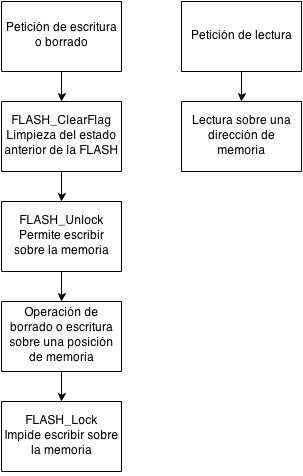
\includegraphics[width=0.5\textwidth]{figs/FLASHDiagram.png}
\caption{Flujo de ejecución de las operaciones sobre la memoria FLASH}
\label{fig:FLASHDiagram}
\end{center}
\end{figure}

A continuación se muestran los test realizados junto a un diagrama de flujo que nos proporcione una guía visual sobre las funciones que realiza. \\

\begin{itemize}
\item int test\_unlock\_lock(): Este test prueba a desbloquear la memoria y volver a bloquearla, controlando en todo momento el estado de la memoria por si surge algún error. Podemos ver el diagrama de secuencia e interacción con la biblioteca de la memoria FLASH en la Figura \ref{fig:testLockUnlock}.

\begin{figure}[!h]
\begin{center}
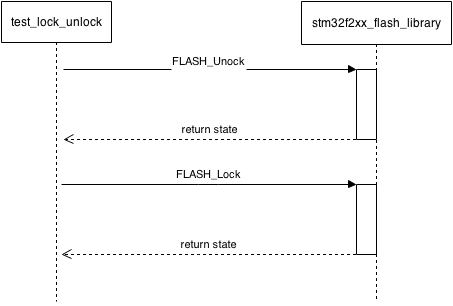
\includegraphics[width=0.5\textwidth]{figs/testLockUnlock.png}
\caption{Diagrama de secuencia e interacción entre el test de \textit{Unlock/Lock} y la biblioteca de acceso a la FLASH}
\label{fig:testLockUnlock}
\end{center}
\end{figure}

\item int test\_flash\_program\_example(): Este test prueba a desbloquear la memoria, resetear el sector, escribir y leer de memoria, controlando en todo momento el estado de la memoria por si sirge algun error. Podemos ver el diagrama de secuencia e interacción con la biblioteca de la memoria FLASH en la Figura \ref{fig:testLockUnlock}. Este test es un ejemplo proporcionado por el fabricante.

\begin{figure}[!h]
\begin{center}
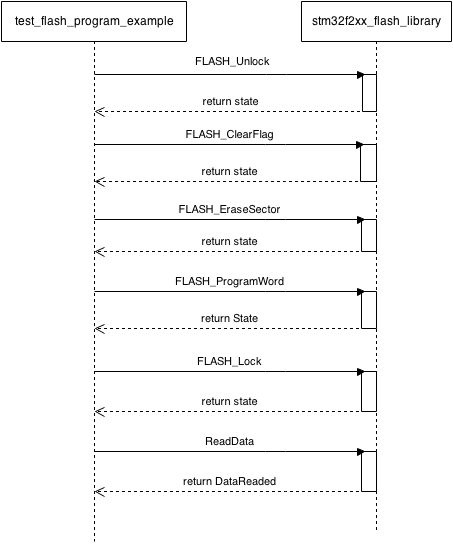
\includegraphics[width=0.5\textwidth]{figs/test_flash_program_example.png}
\caption{Diagrama de secuencia e interacción entre el test de ejemplo  y la biblioteca de acceso a la FLASH}
\label{fig:test_flash_program_example}
\end{center}
\end{figure}

\item int diskRead(uint32\_t address, BYTE *buff, UINT count): Este test prueba a leer de memoria, controlando en todo momento el estado de la memoria por si surge algún error. Podemos ver el diagrama de secuencia e interacción con la biblioteca de la memoria FLASH en la Figura \ref{fig:diskRead}.

\begin{figure}[!h]
\begin{center}
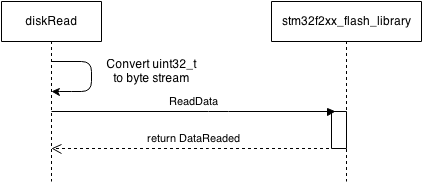
\includegraphics[width=0.5\textwidth]{figs/diskRead.png}
\caption{Diagrama de secuencia e interacción entre el test de lectura y la biblioteca de acceso a la FLASH}
\label{fig:diskRead}
\end{center}
\end{figure}

\item int diskWrite(uint32\_t address, const BYTE *buff, UINT count): Este test prueba a escribir en memoria, controlando en todo momento el estado de la memoria por si surge algún error. Podemos ver el diagrama de secuencia e interacción con la biblioteca de la memoria FLASH en la Figura \ref{fig:diskWrite}.

\begin{figure}[!h]
\begin{center}
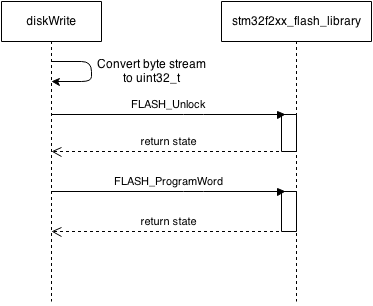
\includegraphics[width=0.5\textwidth]{figs/diskWrite.png}
\caption{Diagrama de secuencia e interacción entre el test de escritura y la biblioteca de acceso a la FLASH}
\label{fig:diskWrite}
\end{center}
\end{figure}

\item int test\_write\_read(): Este test es una combinación de los test de escritura y lectura y comprobando que se escriben y leen los mismos datos. En este test no se detalla el diagrama de secuencia ya que las interacciones con la biblioteca de acceso a la FLASH son las mismas que los test citados.
\end{itemize}


\section{Análisis del acceso al GPS}
\label{obj4}
Como se ha visto antes, para la comunicación y gestión del GPS se utilizan los puertos correspondientes a la USART 3, a la que está conectado. En este apartado se definen los métodos utilizados para la inicialización y lectura de datos del dispositivo GPS.\\

En esta tarea también se ha utilizado uno de los leds, para tener certeza que se está ejecutando correctamente, que se apagará antes de parsear un mensaje y se encenderá cuando se haya parseado correctamente.\\

El dispositivo GPS necesita una inicialización mediante la configuración de la USART a la que está conectado para poder realizar la comunicación con él correctamente. Además necesita que se haya configurado previamente el reloj del sistema ya que es uno de los requisitos de la USART para establecer la comunicación. En la Figura \ref{fig:GPSDiagram} se puede ver el flujo de ejecución del acceso al dispositivo GPS.\\

\begin{figure}[!h]
\begin{center}
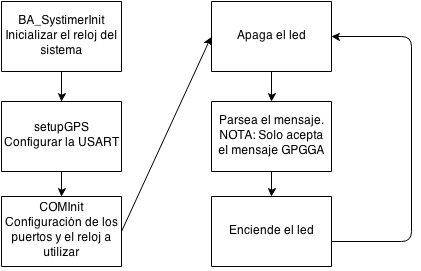
\includegraphics[width=0.5\textwidth]{figs/GPSDiagram.png}
\caption{Flujo de ejecución de las operaciones de acceso al GPS}
\label{fig:GPSDiagram}
\end{center}
\end{figure}

No se dispone de forma de comprobar que los datos del GPS son correctos salvo teniendo otro dispositivo GPS cercano y comprobando los datos, o utilizando alguna herramienta de cartografía como puede ser Google Maps. Por este motivo en este punto no se realizan test de programación.\\

A continuación se va listar los métodos necesarios para inicializar el GPS y lectura de los datos, junto con un diagrama de secuencia para entender cómo se hace y con qué componentes interacciona. \\

\begin{itemize}
\item Inicializar Hardware: En este método se inicializa el hardware del GPS, se configura el reloj del sistema, necesario para que se establezca correctamente la comunicación con el dispositivo y se configuran los puertos de la \acs{USART} utilizada. Se puede ver un diagrama de secuencia e interacción con las bibliotecas de funciones del sistema en la Figura \ref{fig:initGPS}.\\

\begin{figure}[!h]
\begin{center}
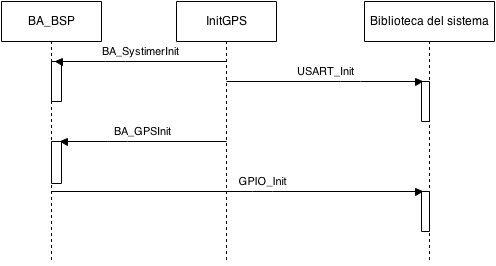
\includegraphics[width=0.5\textwidth]{figs/initGPS.png}
\caption{Diagrama de secuencia e interacción de las operaciones de inicialización del dispositivo GPS}
\label{fig:initGPS}
\end{center}
\end{figure}

\item ParsearDatosGPS: En este método se parsean los datos del GPS para que reconozca únicamente los mensajes definidos en el apartado \ref{obj1}. Este método se ejecuta en bucle, cuando se integre la parte del Sistema de Archivos se escribirán los mensajes válidos en un fichero. Para la lectura de datos utiliza la función implementada en los drivers del sistema \textit{BA\_GPS\_Receive}. Se puede ver un diagrama de secuencia e interacción con las bibliotecas de funciones del sistema en la Figura \ref{fig:parserGPS}.\\

\begin{figure}[!h]
\begin{center}
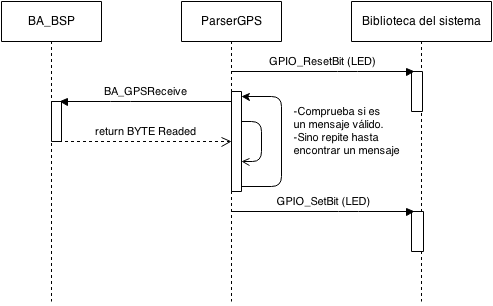
\includegraphics[width=0.5\textwidth]{figs/parserGPS.png}
\caption{Diagrama de secuencia e interacción de las operaciones de lectura y parseo de datos del GPS}
\label{fig:parserGPS}
\end{center}
\end{figure}

\end{itemize}

\section{Implementación de un Sistema de Ficheros}
\label{obj5}

\subsection{Introducción y evaluación de alternativas}
Un sistema de archivos es necesario para proporcionar una capa de abstracción en el acceso a la memoria y el almacenamiento de datos. \\

La implementación de un sistema de ficheros en un sistema empotrado debe ser, como el resto de componentes, lo más eficiente posible. Como los sistemas de archivos llevan muchos tiempo entre nosotros y hay muchas y diferentes alternativas se ha pensado como primera opción utilizar un sistema FAT por su simplicidad.\\

Es necesario considerar los requisitos de la memoria FLASH:
\begin{itemize}
\item 1 MByte de memoria.
\item La memoria está dividida en 11 sectores de diferentes tamaños, desde 16 KBytes hasta 128 KBytes.
\item La granularidad mínima del borrado de la memoria, necesario para poder sobreescribir, es a nivel de sector físico y se pierde toda la información almacenada.
\item La memoria del programa está escrita en la memoria FLASH, por lo que no tenemos disponible toda la capacidad de la memoria para el sistema de archivos.\\
\end{itemize}

Después de estudiar el tema se descartó el uso de un sistema FAT o cualquiera conocido ya que todos funcionan con una granularidad mínima de un sector físico y en este sistema no sirven ya que, como se ha dicho anteriormente, solo se dispone de 11 sectores físicos y además con un tamaño demasiado grande (128 KBytes) en comparación con el tamaño de sector habitual de este tipo de memorias (512 Bytes).\\

\subsection{Diseño del sistema de archivos}

Para crear un sistema de archivos es necesaria una tabla con los descriptores de archivos que nos proporcionen cierta información como puede ser el nombre, necesario para realizar la búsqueda, y la dirección de inicio.\\

Se ha decidido que, por simplicidad y para evitar fragmentación interna, el almacenamiento de los archivos en memoria sea de manera secuencial. Con esto surge un problema debido a que tener varios archivos en memoria implica que cada archivo tiene un límite máximo. Para solucionar el problema mencionado se ha definido un número máximo de ficheros, ya que para este sistema se necesita únicamente uno para datos de configuración y otro para almacenamiento de log, o varios si se desea discriminar por fuentes de datos.\\

La tabla de descriptores se ha definido de la siguiente forma:

\begin{itemize}
\item Un byte de validez, puesto todo a 1 por defecto ya que solo se puede cambiar el valor a 0. Para ver si una entrada es válida basta con comprobar el byte de validez y que la entrada en la tabla no tenga vacío el campo del nombre.
\item El nombre es una cadena de bytes que codifica el nombre.
\item La dirección de inicio será la dirección donde empieza el fichero.
\item La dirección de fin será la siguiente posición de memoria consecutiva a la última posición escrita. \\
\end{itemize}

A partir de estos elementos es necesario ahora definir el tamaño de un sector lógico para facilitar las tareas de lectura y escritura. Partiendo de lo anterior, y de las posibilidades que ofrece la biblioteca de funciones de acceso a la memoria FLASH, es necesario definir un sector lógico de un tamaño múltiplo de una palabra de datos (32 bits o 4 bytes) y del tamaño suficiente para albergar una entrada completa de la tabla de descriptores. El tamaño de cada sector lógico se ha establecido a 16 bytes, pero es configurable.\\

Con un sector lógico de 16 bytes cada entrada de la tabla de descripciones tiene la siguiente estructura: 1 Byte de validez, 7 Bytes de codificación del nombre, 4 Bytes para codificar la dirección de inicio y 4 Bytes para codificar la dirección de fin.\\

Para facilitar la tarea de reconocer que existe un sistema de archivos escrito en memoria cuando montamos el sistema, el primer sector lógico contiene una cadena de texto fácilmente identificable: "FS CORRECTO".\\

En la Tabla \ref{tab:file_descr} \footnote {El byte de validez con valor 255 corresponde con el número en binario 1111, el número 4294967295 corresponde con el número binario 1111 1111 1111 1111.} se puede ver un ejemplo de los datos que podría contener la tabla de descriptores de archivos.\\

\begin{table}[h!]
\centering

\begin{tabular}{p{.15\textwidth}p{.2\textwidth}p{.2\textwidth}p{.2\textwidth}}
\tabheadformat
  \tabhead{Validez}   &
  \tabhead{Nombre}      &
  \tabhead{Dirección de inicio}  &
  \tabhead{Dirección de fin}      \\
\hline
255 & archivo & 2048 & 2184 \\ \hline
255 & ex1.txt & 4112 & 4140 \\ \hline
255 & 1111111 & 4294967295 & 4294967295 \\ 

% \\ 
\hline
\end{tabular}
\caption {Ejemplo de datos de la tabla de descriptores de archivos}
\label{tab:file_descr}
\end{table}

Una entrada en la tabla de descriptores de archivo es válida si el byte de validez tiene un valor de 255 y la dirección de inicio y el nombre tienen valores válidos.\\

Para solucionar el problema de que poder escribir un dato en una posición ya utilizada sin antes realizar una operación de Erase en todo el sector, se creará una nueva tarea que comprobará cada cierto tiempo el uso del sistema de archivos utilizado y, si está lo suficientemente completo, creará un nuevo sistema de archivos vacío en otro sector y será el que se utilice desde ese momento en adelante hasta que sea necesario volver a cambiar el sector físico donde tenemos el sistema de archivos.\\

\subsection{Definición de la biblioteca de acceso al Sistema de Archivos}

La biblioteca de funciones del Sistema de Archivos desarrollado se estructura en dos capas bien diferenciadas: 1)la capa del sistema de archivos propiamente dicha y 2) la capa de abstracción del hardware que ofrece simplicidad a la hora de realizar diversas operaciones sobre la memoria FLASH.\\

A continuación se listan las funciones del Sistema de Archivos desarrollado y las tareas que realiza cada una, así como un diagrama de secuencia de cada una para explicar cómo funcionan internamente y las interacciones con las diferentes capas de abstracción del sistema.\\


\begin{itemize}
\item f\_mount: Crea la estructura de datos necesaria para almacenar los datos del sistema de archivos y le los datos del sistema de archivos del disco. Comprueba si hay un sistema de archivos correcto y extrae los ficheros de la tabla de descriptores. Se puede ver el diagrama de secuencia de esta función en la Figura \ref{fig:fmount}.\\

\begin{figure}[!h]
\begin{center}
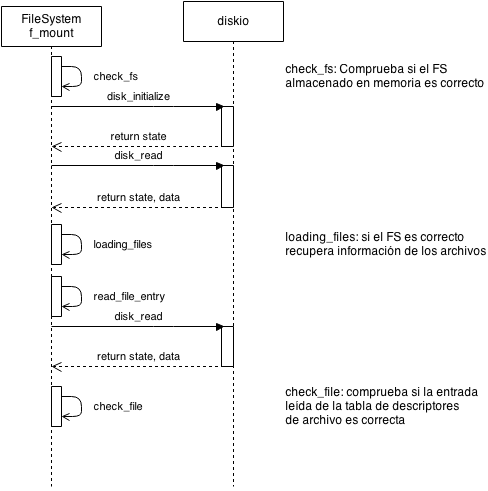
\includegraphics[width=0.5\textwidth]{figs/fmount.png}
\caption{Diagrama de secuencia e interacción de la operación f\_mount del Sistema de Archivos}
\label{fig:fmount}
\end{center}
\end{figure}

\item f\_mkfs: Crea el sistema de archivos, lo configura y escribe en el disco lo que necesite. Se puede ver el diagrama de secuencia de esta función en la Figura \ref{fig:fmkfs}.\\

\begin{figure}[!h]
\begin{center}
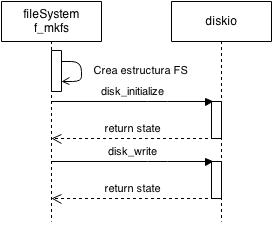
\includegraphics[width=0.5\textwidth]{figs/fmkfs.png}
\caption{Diagrama de secuencia e interacción de la operación f\_mkfs del Sistema de Archivos}
\label{fig:fmkfs}
\end{center}
\end{figure}

\item f\_open: Dependiendo del modo de apertura abrirá un archivo existente o creará uno nuevo. Se puede ver el diagrama de secuencia de esta función en la Figura \ref{fig:fopen}.\\

\begin{figure}[!h]
\begin{center}
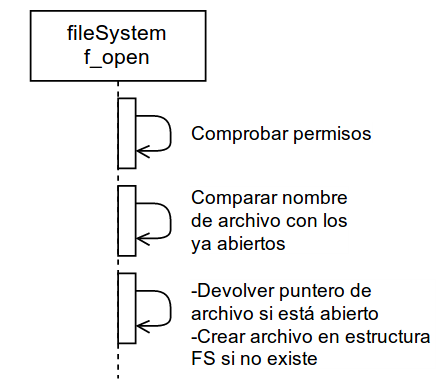
\includegraphics[width=0.5\textwidth]{figs/fopen.png}
\caption{Diagrama de secuencia e interacción de la operación f\_open del Sistema de Archivos}
\label{fig:fopen}
\end{center}
\end{figure}

\item f\_close: Cerrará el archivo. En este momento se vuelcan en memoria todos los datos no guardados que se encuentren en el buffer de escritura y se actualizará la tabla de descriptores de archivo. Se puede ver el diagrama de secuencia de esta función en la Figura \ref{fig:fclose}.\\

\begin{figure}[!h]
\begin{center}
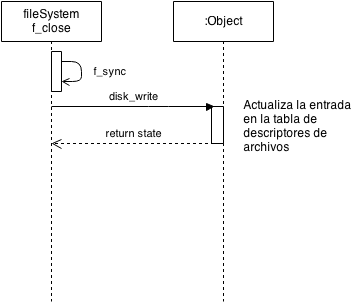
\includegraphics[width=0.5\textwidth]{figs/fclose.png}
\caption{Diagrama de secuencia e interacción de la operación f\_close del Sistema de Archivos}
\label{fig:fclose}
\end{center}
\end{figure}

\item f\_read: Se leerá de disco el tamaño en bytes especificado al invocar la función. Se puede ver el diagrama de secuencia de esta función en la Figura \ref{fig:fread}.\\

\begin{figure}[!h]
\begin{center}
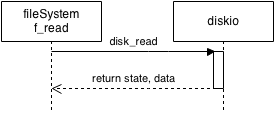
\includegraphics[width=0.5\textwidth]{figs/fread.png}
\caption{Diagrama de secuencia e interacción de la operación f\_read del Sistema de Archivos}
\label{fig:fread}
\end{center}
\end{figure}

\item f\_write: Se escribirá en disco el tamaño en bytes especificado al invocar la función. Si el tamaño especificado es menor que el tamaño del buffer (el mismo tamaño que el sector) entonces no se escribirá hasta que el buffer de escritura se llene. Se puede ver el diagrama de secuencia de esta función en la Figura \ref{fig:fwrite}.\\

\begin{figure}[!h]
\begin{center}
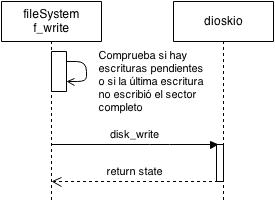
\includegraphics[width=0.5\textwidth]{figs/fwrite.png}
\caption{Diagrama de secuencia e interacción de la operación f\_write del Sistema de Archivos}
\label{fig:fwrite}
\end{center}
\end{figure}

\item f\_lseek: Cambia el puntero de lectura a la dirección especificada. Cambia el valor del campo correspondiente en la estructura de datos que representa a un archivo.\\


\item f\_sync: Fuerza las escrituras pendientes que haya. Se puede ver el diagrama de secuencia de esta función en la Figura \ref{fig:fsync}.\\

\begin{figure}[!h]
\begin{center}
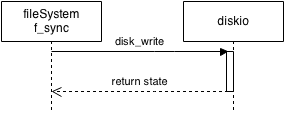
\includegraphics[width=0.5\textwidth]{figs/fsync.png}
\caption{Diagrama de secuencia e interacción de la operación f\_sync del Sistema de Archivos}
\label{fig:fsync}
\end{center}
\end{figure}

\item f\_truncateStart: Modificará la posición de inicio de un archivo. En la práctica consiste en el borrado de la parte más antigua del fichero. Cambia el valor del campo correspondiente en la estructura de datos que representa a un archivo y se actualizará en la tabla de descriptores de archivo cuando éste se cierre.\\


\item f\_getfree: Obtiene el mínimo de los tamaños disponibles para escritura de archivos. Se puede ver el diagrama de secuencia de esta función en la Figura \ref{fig:fgetfree}.\\

\begin{figure}[!h]
\begin{center}
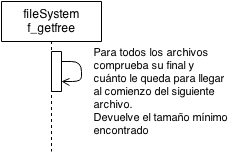
\includegraphics[width=0.5\textwidth]{figs/fgetfree.png}
\caption{Diagrama de secuencia e interacción de la operación f\_getfree del Sistema de Archivos}
\label{fig:fgetfree}
\end{center}
\end{figure}

\item reset\_sector: Realiza una operación de \textit{Reset} (o \textit{Erase}) en el sector, dejándolo preparado para nuevas escrituras. Se puede ver el diagrama de secuencia de esta función en la Figura \ref{fig:resetsector}.

\begin{figure}[!h]
\begin{center}
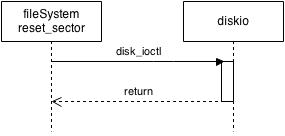
\includegraphics[width=0.5\textwidth]{figs/resetsector.png}
\caption{Diagrama de secuencia e interacción de la operación reset\_sector del Sistema de Archivos}
\label{fig:resetsector}
\end{center}
\end{figure}

\item change\_sector: Cambia el sector físico en el que se encuentra el sistema de archivos. Realiza todos los pasos necesarios para crear un sistema de archivos en otro sector especificado en el archivo de configuración. Resetea el sector, crea el sistema, lo monta y, si se le indicamos, hace un \textit{backup} de los archivos de un sistema en el otro. Se puede ver el diagrama de secuencia de esta función en la Figura \ref{fig:changesector}.\\

\begin{figure}[!h]
\begin{center}
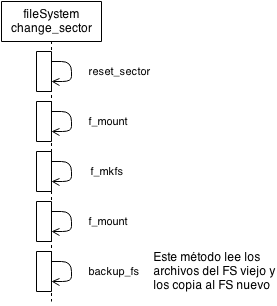
\includegraphics[width=0.5\textwidth]{figs/changesector.png}
\caption{Diagrama de secuencia e interacción de la operación change\_sector del Sistema de Archivos}
\label{fig:changesector}
\end{center}
\end{figure}


\end{itemize}

Para separar la gestión del sistema de archivos de los accesos a disco y simplificar la programación, el sistema de archivos propuesto ha sido programado sobre una biblioteca de acceso a la memoria FLASH que tiene las siguientes funciones:

\begin{itemize}
\item disk\_initialize: Inicializará la memoria FLASH. En la práctica la operación consiste en limpiar todos los registros de estado. Se puede ver el diagrama de secuencia de esta función en la Figura \ref{fig:diskinitialize}.\\

\begin{figure}[!h]
\begin{center}
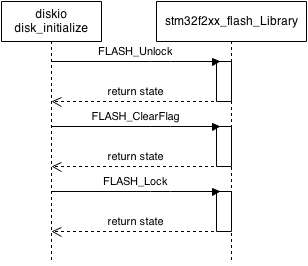
\includegraphics[width=0.5\textwidth]{figs/diskinitialize.png}
\caption{Diagrama de secuencia e interacción de la operación disk\_initialize de la capa de abstracción de la memoria FLASH}
\label{fig:diskinitialize}
\end{center}
\end{figure}

\item disk\_status: Devuelve el estado actual de la memoria FLASH. Se puede ver el diagrama de secuencia de esta función en la Figura \ref{fig:diskstatus}.\\

\begin{figure}[!h]
\begin{center}
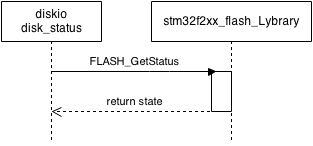
\includegraphics[width=0.5\textwidth]{figs/diskstatus.png}
\caption{Diagrama de secuencia e interacción de la operación disk\_status de la capa de abstracción de la memoria FLASH}
\label{fig:diskstatus}
\end{center}
\end{figure}

\item disk\_read: Lee, a partir de una dirección de memoria dada, la cantidad de sectores especificados. Se puede ver el diagrama de secuencia de esta función en la Figura \ref{fig:diskRead}.\\

\item disk\_write: Escribe, a partir de una dirección de memoria dada, la cantidad de setores especificados. Se puede ver el diagrama de secuencia de esta función en la Figura \ref{fig:diskWrite}.\\

\item disk\_ioctl: Agrupa algunas funciones de control, se especificará en uno de los parámetros de entrada qué queremos hacer. Las operaciones soportadas serán: 
\begin{itemize}

\item CTRL\_SYNC: Esperará hasta que todas las operaciones sobre la FLASH se hayan completado.
\item GET\_SECTOR\_COUNT: Devolverá el número total de sectores presentes en el sistema de archivos.
\item GET\_SECTOR\_SIZE: Devolverá el tamaño de los sectores del sistema de archivos.
\item CTRL\_ERASE\_SECTOR: Realizará la operación de \textit{Reset/Erase} sobre el sector especificado.\\
\end{itemize} 
Se puede ver el diagrama de secuencia de esta función en la Figura \ref{fig:diskioctl}.\\

\begin{figure}[!h]
\begin{center}
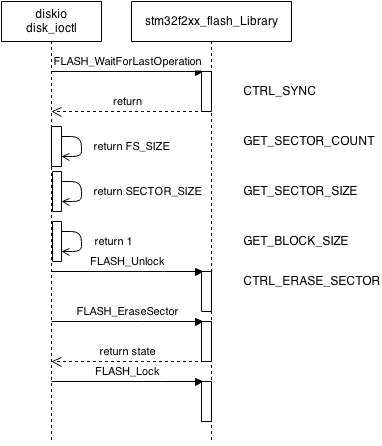
\includegraphics[width=0.5\textwidth]{figs/diskioctl.png}
\caption{Diagrama de secuencia e interacción de la operación disk\_ioctl de la capa de abstracción de la memoria FLASH}
\label{fig:diskioctl}
\end{center}
\end{figure}

\end{itemize}


\section{Programación y configuración del Sistema Operativo en Tiempo Real FreeRTOS}
\label{obj6}
En un sistema empotrado el uso de un sistema operativo es algo crítico ya que, aunque ayuda con la programación del sistema proporcionándonos una capa de abstracción para el manejo de tareas y cambios de contexto, los recursos que consume pueden ser considerables.\\

A continuación se expondrán una serie de características inherentes a todo sistema operativo de tiempo real y algunos de sus inconvenientes.\\

\begin{itemize}
\item Cada tarea tiene su propio estado y se ejecuta como un programa indepentiente.
\item La ejecución de las tareas se maneja mediante el planificador del Sistema Operativo.
\item Cuando ocurre una interrupción se suspende la ejecución de una tarea y se ejecuta la tarea asociada a la interrupción.
\item Los mecanismos de coordinación entre tareas son las interrupciones, los semáforos y las colas de mensajes. Hay que tener especial cuidado ya que pueden darse condiciones de carrera\footnote{Una condición de carrera sucede cuando varios procesos acceden a un mismo recurso y el resultado de las operaciones cambia dependiendo del orden de ejecución de las mismas.}.
\item Cada tarea tiene una zona reservada de memoria, o pila, y puede desbordarse si no se ha reservado suficiente espacio.\\
\end{itemize}

\subsection{Gestión de la memoria RAM}
La gestión de la memoria RAM, como se ha comentado anteriormente, es esencial para el correcto funcionamiento del sistema operativo y las tareas. En la Figura \ref{fig:RAM} se puede ver la disposición en memoria de los datos que se describen a continuación.
\begin{itemize}
\item En la parte inferior de la memoria se guarda la pila de cada tarea.
\item En la parte superior de la memoria se guarda la pila del sistema.
\item En la pila del sistema se guarda, principalmente, la pila de interrupciones.
\item La pila de datos es donde se guardan todos los datos compartidos.\\
\end{itemize}

\begin{figure}[!h]
\begin{center}
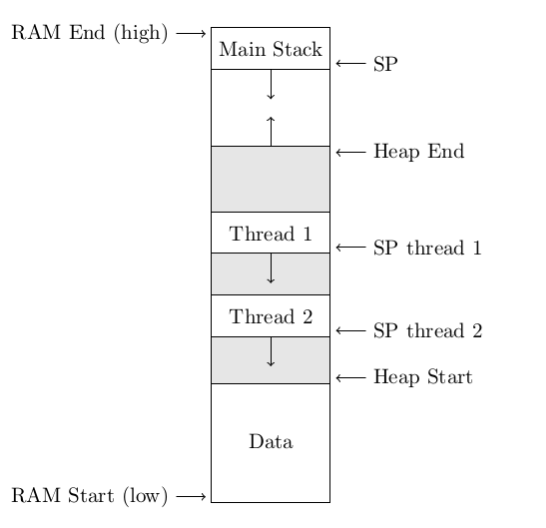
\includegraphics[width=0.4\textwidth]{figs/RAM.png}
\caption{Disposición de la memoria de las tareas en memoria RAM}
\label{fig:RAM}
\end{center}
\end{figure}

Para la gestión de la memoria RAM que utilizan las tareas se ha optado por la utilización de la opción 2 que proporciona FreeRTOS en el archivo \textit{heap2.c}, que permite liberar bloques usados para volver a ser utilizados posteriormente. La cantidad total de espacio dinámico es determinado en el archivo de configuración. Esta configuración tiene el inconveniente de que no es capaz de agrupar en una porción de memoria mayor partes adyacentes que hayan sido liberadas, por lo que solo podrán utilizarse para tareas o estructuras de datos de igual o menor tamaño, incrementando la fragmentación interna. En el caso de la gestión de tareas de este TFG no existe problema con la fragmentación interna, ya que no se eliminan tareas y las estructuras de datos son siempre del mismo tamaño.\\

\subsection{Gestión de las tareas}
Las tareas, o Threads, que maneja FreeRTOS son con prioridad de apropiación, es decir, que cualquier tarea con mayor prioridad va a ejecutarse si está preparada. Las tareas con igual prioridad son ejecutadas alternándose entre sí con un tiempo de \textit{poolling} determinado.\\

En la Figura \ref{fig:FSMThreads} se puede ver la máquina de estados de cada tarea. A continuación se pasan a describir los estados y cómo pasan de uno a otro.
\begin{itemize}
\item Cuando se crea una tarea su estado 0.
\item Existe una única una tarea con estado 2.
\item Una tarea ejecutándose puede ser pausada y volver al estado 1.
\item Una tarea ejecutándose puede ser bloqueada y pasar al estado 3.
\item Una tarea bloqueada puede pasar al estado 1.
\item El estado suspendido de FreeRTOS se utiliza con la llamada vTaskSuspendAll(). Esta función pasa todas las tareas a estado suspendido excepto aquella que ha invocado la función.\\
\end{itemize}

\begin{figure}[!h]
\begin{center}
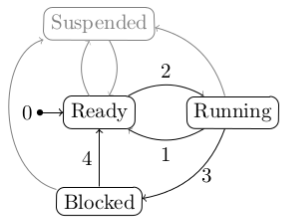
\includegraphics[width=0.3\textwidth]{figs/ThreadsStates.png}
\caption{Máquina de estados de las tareas}
\label{fig:FSMThreads}
\end{center}
\end{figure}

Cada tarea es creada con una función a ejecutar, un nombre, un tamaño de pila, algunos parámetros opcionales, una prioridad y la localización del manejador de la tarea. A partir de aquí el sistema operativo crea la estructura necesaria y la coloca en memoria donde corresponda. El tamaño de la pila es crítico ya que si es demasiado pequeño es probable que haya desbordamiento y si es demasiado grande puede que no exista espacio para otras tareas. Como dato, utilizar bibliotecas de funciones incrementa significativamente el tamaño necesario en la pila al tener que almacenar funciones que nunca van a ser utilizadas.\\

Para la gestión del tiempo en que todas las tareas puedan estar bloqueadas esperando recursos, FreeRTOS crea una tarea vacía con la menor prioridad posible.\\

Los mecanismos de sincronización entre tareas proporcionan una interfaz segura para administrar los recursos compartidos, de manera que cuando una tarea pide un recurso el planificador éste es asignado si está libre o es bloqueada hasta que otra tarea lo libere.\\

FreeRTOS soporta también colas de mensajes para pasar información de una tarea a otra. Para crearla es necesario especificar un identificador, el tamaño máximo de un mensaje y el máximo de mensajes que puede almacenar. Los mensajes son añadidos a una cola de mensajes copiando la referencia, por lo que consumen memoria de la tarea que los envía, y deben especificar un tiempo máximo de espera para ser atendidos.\\

Sobre las interrupciones FreeRTOS las trata añadiéndolas a una cola de mensajes, que será tratada por la tarea correspondiente.\\

\subsection{Funciones necesarias para construir una aplicación con FreeRTOS}

En el Listado \ref{code:bibFreeRTOS} podemos ver las funciones de FreeRTOS que se necesitan utilizar para la realización de este TFG, junto con una pequeña explicación de cada una.\\

\begin{listing}[
  %float=ht,
  language = C,
  rulesepcolor = \color{black},
  caption  = {Funciones necesarias para construir una aplicación con FreeRTOS},
  label    = code:bibFreeRTOS]
  
 /* Creacion de una tarea, necesitamos especificar la funcion   *
  * a lanzar, el nombre de la tarea, el tamanyo de la pila,     *
  * parametros extra si los hubiese, la prioridad y el puntero  *
  * donde quieras que se devuelva el manejador de la tarea.     */
 BaseType_t xTaskCreate( 
                            TaskFunction_t pvTaskCode, 
                            const char * const pcName, 
                            unsigned short usStackDepth, 
                            void *pvParameters, 
                            UBaseType_t uxPriority, 
                            TaskHandle_t *pvCreatedTask 
                          );
                          
 /* Creacion de una cola de mensajes, necesitamos especificar la *
  * longitud de la cola y el tamanyo maximo de mensaje.          */              
 QueueHandle_t xQueueCreate( 
                            UBaseType_t uxQueueLength, 
                            UBaseType_t uxItemSize 
                          );
                          
 /* Envio de un mensaje a una cola, se debe especificar la cola  *
  * de mensajes objetivo, la variable o estructura a enviar y    *
  * el tiempo maximo de bloqueo esperando sincronizacion.        */                          
 BaseType_t xQueueSend( 
                            QueueHandle_t xQueue, 
                            const void * pvItemToQueue, 
                            TickType_t xTicksToWait 
                         );
                         
 /* Recepcion de un mensaje a una cola, se debe especificar la   *
  * cola de mensajes objetivo, la variable o estructura a enviar *
  * y el tiempo maximo de bloqueo esperando sincronizacion.      */                         
 BaseType_t xQueueReceive(
                            QueueHandle_t xQueue,
                            void *pvBuffer,
                            TickType_t xTicksToWait
                         );
\end{listing}

\section{Diseño y programación del sistema final}
\label{obj7}

En las secciones anteriores ya hemos definido el sistema de archivos y cómo utilizarlo (Sección \ref{obj5}), el acceso al GPS y cómo utilizarlo (Sección \ref{obj4}) y cómo funciona FreeRTOS (Sección \ref{obj6}). En esta sección se unifican los módulos individuales ya creados e integran en el sistema final objetivo de este TFG.\\

En la Figura \ref{fig:allSystem} podemos ver el diagrama de componentes del Sistema final, dividido en capas según la funcionalidad de los componentes.\\

\begin{figure}[!h]
\begin{center}
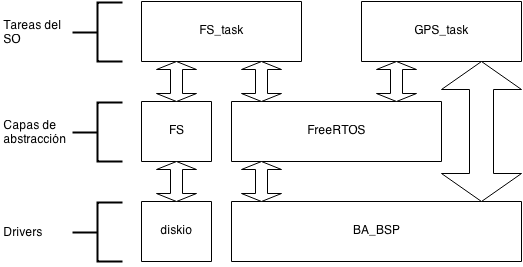
\includegraphics[width=0.8\textwidth]{figs/allSystem.png}
\caption{Diagrama de componentes del Sistema final}
\label{fig:allSystem}
\end{center}
\end{figure}

El sistema final constará de dos tareas definidas en FreeRTOS, una para la gestión de la memoria y otra para la gestión del GPS. La comunicación y sincronización entre ambas será realizada a través de una cola de mensajes de FreeRTOS. El problema de concurrencia a afrontar entre estas dos tareas es el problema del productor-consumidor. Para tener alguna interacción con el usuario el sistema va a encender un led verde cada vez que el GPS ofrezca un dato válido y un led rojo cada vez que consuma ese dato y lo escriba en el sistema de archivos.\\

\subsection{Tarea encargada de acceso al GPS}

La tarea encargada de gestionar el GPS va directamente sobre funciones de la biblioteca de funciones proporcionada por el fabricante.\\

La función que ejecuta la tarea es GPSTaskFunc, que nada más ejecutarse inicializa el componente hardware del GPS y a continuación ejecuta permanentemente la tarea de parsear los datos y enviarlos a la cola de mensajes.\\

Las funciones de inicialización, comunicación e identificación de los mensajes del dispositivo GPS son los descritos en el apartado \ref{obj4}, salvo con la diferencia que la función \textit{parserGPS} envía los mensajes válidos a la cola de mensajes con la que se comunica con la tarea encargada de gestionar la memoria.\\

El código fuente de la tarea encargada de gestionar el GPS se puede encontrar en el Anexo .

\subsection{Tarea encargada de acceso a la memoria FLASH}

La tarea encargada de gestionar la memoria se encuentra sobre una capa de abstracción del sistema de archivos, a su vez sobre una capa de abstracción de acceso al hardware y sobre la biblioteca de funciones proporcionada por el fabricante.\\

La función que ejecuta la tarea es FSTaskFunc. Nada más ejecutarse inicializa el componente hardware del sistema de archivos, que básicamente consiste en realizar una función de \textit{reset}, creación y montaje de un sistema de archivos sobre el sector especificado en los archivos de configuración. A continuación ejecuta permanentemente la tarea que consume datos de la cola de mensajes y los inserta en un fichero.\\
 

























